
%% USE one of these:
%% * the first when using pdflatex, which directly typesets your document in the
%%   chosen pdf/a format and you want to publish your thesis online,

%% * the second when you want to print your thesis to bind it, or
%% * the third when producing a ps file and a pdf/a from it.
%%
%\documentclass[english, 12pt, a4paper, elec, utf8, a-1b, online]{aaltothesis}
%\documentclass[english, 12pt, a4paper, elec, utf8, a-1b]{aaltothesis}
%\documentclass[english, 12pt, a4paper, elec, dvips, online]{aaltothesis}
\documentclass[english,12pt,a4paper,pdftex,sci,utf8]{aaltothesis} % ITSE LISÄTTY. pdfx.sty vanha.

%% Use the following options in the \documentclass macro above:
%% your school: arts, biz, chem, elec, eng, sci
%% the character encoding scheme used by your editor: utf8, latin1
%% thesis language: english, finnish, swedish
%% make an archiveable PDF/A-1b, PDF/A-2b or PDF/A-3b compliant file: a-1b,
%%                    a-2b, a-3b
%%                    (a normal pdf is produced without the a-*b option)
%% typeset in symmetric layout and blue hypertext for online publication: online
%%            (no option is the default, resulting in a wide margin on the
%%             binding side of the page and black hypertext)
%% two-sided printing: twoside (default is one-sided printing)
%%

\usepackage{bbm} % bold indicator function
\usepackage{graphicx, float} % graphics
\usepackage{ctable} % for tables
\usepackage{hyperref} % for the internal links
\hypersetup{
hidelinks,
bookmarksnumbered=true
}

%% Math fonts, symbols, and formatting
\usepackage{amsfonts,amssymb,amsbsy,amsmath,amsthm}


% Theorems, corollaries and lemmas
\newtheorem{theorem}{Theorem}[section]
\newtheorem{corollary}[theorem]{Corollary}
\newtheorem{lemma}[theorem]{Lemma}
\newtheorem{definition}[theorem]{Definition}

%% Change the school field to specify your school if the automatically set name
%% is wrong
% \university{aalto-yliopisto}
% \school{Sähkötekniikan korkeakoulu}

%% Edit to conform to your degree programme
%%
\degreeprogram{Technical Physics and Mathematics}
%%

%% Your major
%%
\major{Mathematics and Systems Analysis}
%%

%% Major subject code
%%
\code{SCI3029}
%%
 
%% Choose one of the three below
%%
\univdegree{BSc}
%\univdegree{MSc}
%\univdegree{Lic}
%%

%% Your name (self explanatory...)
%%
\thesisauthor{Jaakko Pere}
%%

%% Your thesis title comes here and possibly again together with the Finnish or
%% Swedish abstract. Do not hyphenate the title, and avoid writing too long a
%% title. Should LaTeX typeset a long title unsatisfactorily, you mght have to
%% force a linebreak using the \\ control characters.
%% In this case...
%% Remember, the title should not be hyphenated!
%% A possible "and" in the title should not be the last word in the line, it
%% begins the next line.
%% Specify the title again without the linebreak characters in the optional
%% argument in box brackets. This is done because the title is part of the 
%% metadata in the pdf/a file, and the metadata cannot contain linebreaks.
%%
\thesistitle{Asymptotic Properties of the Hill Estimator}
%\thesistitle[Title of the thesis]{Title of\\ the thesis}
%%

%%
\place{Espoo}
%%

%% The date for the bachelor's thesis is the day it is presented
%%
\date{23.8.2018}
%%

%% Thesis supervisor
%% Note the "\" character in the title after the period and before the space
%% and the following character string.
%% This is because the period is not the end of a sentence after which a
%% slightly longer space follows, but what is desired is a regular interword
%% space.
%%
\supervisor{Ph.D  Pauliina Ilmonen}
%%

%% Advisor(s)---two at the most---of the thesis. Check with your supervisor how
%% many official advisors you can have.
%%
%\advisor{Prof.\ Pirjo Professor}
\advisor{M.Sc Matias Heikkilä}
%\advisor{MSc Sarah Scientist}
%%

%% Aaltologo: syntax:
%% \uselogo{aaltoRed|aaltoBlue|aaltoYellow|aaltoGray|aaltoGrayScale}{?|!|''}
%% The logo language is set to be the same as the thesis language.
%%
\uselogo{aaltoRed}{?}
%%

%% The English abstract:
%% All the details (name, title, etc.) on the abstract page appear as specified
%% above.
%% Thesis keywords:
%% Note! The keywords are separated using the \spc macro
%%
\keywords{Hill estimator\spc extreme value theory\spc asymptotic properties\spc statistics}
%%

%% The abstract text. This text is included in the metadata of the pdf file as well
%% as the abstract page.
%%
\thesisabstract{
We review the proof of the Hill estimator's consistency. Properties of the regularly varying functions play a crucial role in the theory. Consistency is also studied using simulations. Other properties of the Hill estimator such as asymptotic normality are also reviewed briefly.
}

%% Copyright text. Copyright of a work is with the creator/author of the work
%% regardless of whether the copyright mark is explicitly in the work or not.
%% You may, if you wish, publish your work under a Creative Commons license (see
%% creaticecommons.org), in which case the license text must be visible in the
%% work. Write here the copyright text you want. It is written into the metadata
%% of the pdf file as well.
%% Syntax:
%% \copyrigthtext{metadata text}{text visible on the page}
%% 
%% In the macro below, the text written in the metadata must have a \noexpand
%% macro before the \copyright special character, and macros (\copyright and
%% \year here) must be separated by the \ character (space chacter) from the
%% text that follows. The macros in the argument of the \copyrighttext macro
%% automatically insert the year and the author's name. (Note! \ThesisAuthor is
%% an internal macro of the aaltothesis.cls class file).
%% Of course, the same text could have simply been written as
%% \copyrighttext{Copyright \noexpand\copyright\ 2018 Eddie Engineer}
%% {Copyright \copyright{} 2018 Eddie Engineer}
%%
\copyrighttext{Copyright \noexpand\copyright\ \number\year\ \ThesisAuthor}
{Copyright \copyright{} \number\year{} \ThesisAuthor}

%% You can prevent LaTeX from writing into the xmpdata file (it contains all the 
%% metadata to be written into the pdf file) by setting the writexmpdata switch
%% to 'false'. This allows you to write the metadata in the correct format
%% directly into the file thesistemplate.xmpdata.
%\setboolean{writexmpdatafile}{false}

%% All that is printed on paper starts here

\begin{document}

%% Create the coverpage
%%
\makecoverpage

%% Typeset the copyright text.
%% If you wish, you may leave out the copyright text from the human-readable
%% page of the pdf file. This may seem like a attractive idea for the printed
%% document especially if "Copyright (c) yyyy Eddie Engineer" is the only text
%% on the page. However, the recommendation is to print this copyright text.
%%
\makecopyrightpage

%% Note that when writting your thesis in English, place the English abstract
%% first followed by the possible Finnish or Swedish abstract.

%% Abstract text
%% All the details (name, title, etc.) on the abstract page appear as specified
%% above.
%%
\begin{abstractpage}[english]
 \abstracttext{}
\end{abstractpage}

%% The text in the \thesisabstract macro is stored in the macro \abstractext, so
%% you can use the text metadata abstract directly as follows:
%%
%\begin{abstractpage}[english]
%	\abstracttext{}
%\end{abstractpage}



%\newpage


%% Preface
%%
\mysection{Preface}
Simulations were performed using computer resources within the Aalto University School of Science "Science-IT" project.\\

\vspace{5cm}
Otaniemi, 23.8.2018

\vspace{5mm}
{\hfill Jaakko Pere \hspace{1cm}}

%% Force a new page after the preface
%%
\newpage


%% Table of contents. 
%%
\thesistableofcontents


%% Symbols and abbreviations
\mysection{Symbols and Abbreviations}

\subsection*{Symbols}

\begin{tabular}{ll}
$x^*=\sup\{x : F(x)<1\}$  & the right endpoint of the distribution $F$ \\
$\gamma$ & extreme value index \\
$F^{\leftarrow}(y) = \inf\{x:F(x) \geq y \}$ & left-continuous inverse \\
U & the left-continuous inverse of $\frac{1}{1-F}$ \\
$\mathbbm{1}(p)=
\begin{cases}
1 , \textrm{if p is true}\\
0, \textrm{otherwise}
\end{cases}$ & indicator function \\
$X_{i,n}$ & $i$:th order statistic \\
$\lambda$ & Lebesque measure \\
$\lim \sup A_n = \bigcap_{k=1}^{\infty} \bigcup_{n=k}^{\infty} A_n$ & limit supremum of a sequence of sets $A_n$ \\
$RV_{\alpha}$ & the set of regularly varying functions with index $\alpha$ \\
$D(G_{\gamma})$ & the maximum domain of attraction of $G_{\gamma}$ \\
$f \sim g$ & $\lim\limits_{x \rightarrow \infty} f(x)/g(x)=1$ \\
\end{tabular}


\subsection*{Abbreviations}

\begin{tabular}{ll}
cdf         & cumulative distribution function \\
i.d.d.     & independent and identically distributed \\
a.s.         & almost surely\\
\end{tabular}


%% \clearpage is similar to \newpage, but it also flushes the floats (figures
%% and tables).
%%
\cleardoublepage

%% Text body begins. Note that since the text body is mostly in Finnish the
%% majority of comments are also in Finnish after this point. There is no point
%% in explaining Finnish-language specific thesis conventions in English.
%% This text will be translated to English soon.
%%
\section{Introduction}

Heavy-tailed distributions appear in many fields of science such as insurance and finance. For example the loss returns of a speculative asset or insurance are often heavy-tailed and in practice the focus is often on risk evaluation. One example of such data set is Danish fire insurance loss data \cite{mcneil}  \cite{resnickFire}. Further examples are given in \cite{resnick}, \cite{deHaan} and \cite{embrechts}.

Analyzing the tail is challenging since using classical methods, such as empirical quantiles, it is impossible to extrapolate beyond the available data. This motivates the use of Extreme Value Theory (EVT), that provides a rigorous mathematical framework to study extremes. EVT characterizes the behavior of the distribution's tail and tail estimation is often of high practical importance.

One of the possible estimators for extreme value index is the Hill estimator, which was introduced by Bruce M. Hill in 1975 \cite{hill} and remains one of the most used tail estimators for heavy-tailed distributions.
In this article we will review asymptotic properties of the Hill estimator and particularly its consistency.

Regularly varying functions form the mathematical foundation for the theory of heavy-tailed distributions and consequently they play an important role in the theory of the Hill estimator. We carefully review their properties in addition to consistency of the Hill estimator. We also examine consistency of the Hill estimator by performing Monte Carlo simulations. Results for asymptotic normality of the Hill estimator are provided but won’t be discussed in detail.

The rest of the article is organized as follows. Section \ref{backround} gives requisites for the proofs and theory of the Hill estimator including properties of heavy tailed functions. Section \ref{hillEst} represents the main result, which is consistency and necessary lemmas for the proof of the consistency. Simulations are presented in Section \ref{simut} and concluding remarks are given in Section \ref{conclusion}. Lastly, all the proofs and figures are found in Appendixes \ref{proofs} and \ref{figures}.

%\begin{definition}
%\begin{equation*}
%\hat{\gamma} = \frac{1}{k} \sum_{i=0}^{k-1} \log(X_{n-1,n}) - \log(X_{n-k,n}), \quad 1 \leq k \leq n-1
%\end{equation*}
%\end{definition}

%% Leave page number of the first page empty
%% 
\thispagestyle{empty}




%% Opinn\"aytteess\"a jokainen osa alkaa uudelta sivulta, joten \clearpage
%%
%% In a thesis, every section starts a new page, hence \clearpage
\clearpage

\section{Backround}
\label{backround}

\subsection{Fisher-Tippett-Gnedenko Theorem}
\label{domains}

Let $X_1, X_2, ..., X_n$ be i.d.d. random variables with a cdf $F$. Consider the  sample maxima $M_n = \max(X_1, X_2, ..., X_n)$. The limiting behavior of $M_n$ is trivial: Since $X_1, X_2,..., X_3$ are i.d.d.
\begin{gather*}
P(\max(X_1, X_2, ... , X_n) \leq x) = P(X_1 \leq x, X_2 \leq x,..., X_n \leq x) \\ = 
P(X_1 \leq x) P(X_2 \leq x) ... P(X_n \leq x)
=F^n(x).
\end{gather*}
Now,
\begin{gather*}
\lim_{n\to\infty} F^n(x) = 
\begin{cases}
0, x < x^* \\
1, x \geq x^*.
\end{cases}
\end{gather*}



To achieve a nondegerate distribution it is necessary to normalize the sample maxima $M_n$. The Fisher-Tippett-Gnedenko Theorem states that with a suitable normalization a nondegenate distribution is obtained \cite{fisher} \cite{gnedenko}.

\begin{theorem}
There exists real constants $a_n>0$ and $b_n \in \mathbb{R}$ such that 

\begin{equation}
\lim_{n\to\infty} F^n(a_nx + b_n) = G_{\gamma}(ax+b),
\label{fisher}
\end{equation}
where
\begin{equation*}
G_{\gamma}(x)=
\begin{cases}
\exp(-(1 + \gamma x)^{-\frac{1}{\gamma}}), \gamma \neq 0 \\
\exp(-e^{-x}), \gamma = 0,
\end{cases}
\label{mdaEq}
\end{equation*}
for all x with $1+\gamma x > 0$ where $\gamma \in \mathbb{R}$.
\end{theorem}
If F satisfies the Equation \eqref{fisher} for some $\gamma \in \mathbb{R}$ then it is said that F is in the maximum domain of attraction of $G_{\gamma}$, denoted $F \in D(G_{\gamma})$.

We are especially interested in heavy-tailed distributions, i.e. the case $F \in D(G_{\gamma})$, with $\gamma>0$. It turns out that $F$ being heavy-tailed is equivalent to the function $1-F$ being regularly varying with index $-1/ \gamma$. In other words, if the tail function $1-F$ of a distribution is regularly varying then the distribution $F$ is heavy tailed and vice versa. \cite{deHaan}

\begin{theorem}
Cdf F is in the maximum domain of attraction of the extreme value distribution $G_{\gamma}$ with $\gamma>0$ if and only if $x^*=\infty$ and
\begin{equation}
\lim_{t\rightarrow \infty} \frac{1-F(tx)}{1-F(t)} = x^{-\frac{1}{\gamma}}, x>0.
\label{tail}
\end{equation}
\end{theorem}

In addition, \eqref{tail} can be written in a different form in terms of a left-continuous inverse $U=(1/(1-F))^{\leftarrow}$ \cite{deHaan}.

\begin{corollary}
Condition \eqref{tail} is equivalent to
\begin{equation}
\lim_{t \rightarrow \infty} \frac{U(tx)}{U(t)} = x^{\gamma}, x>0.
\label{Utail}
\end{equation}
\end{corollary}

Relation \eqref{Utail} turns out to be easier to work with than \eqref{tail} and thus it is used in furher calculations.
%Above equation implies that U is regularly varying with index $\gamma$ if $F \in D(G_{\gamma>0})$.


\subsection{Regularly Varying Functions}

In Section \ref{domains} we saw that $F \in D(G_{\gamma})$ with $\gamma>0$ and $U$ being regularly varying function are equivalent conditions. Regularly varying functions have some useful properties that are needed for the proof of the Hill estimator's consistency. Let's define regularly varying functions properly \cite{deHaan}:
\begin{definition}
A Lebesque measurable function $f: \mathbb{R}^{+} \rightarrow \mathbb{R}$ that is eventually positive is regularly varying if for some index $\alpha \in \mathbb{R}$,
\begin{equation}
\lim_{x \rightarrow \infty} \frac{f(tx)}{f(t)} = x^{\alpha}, x>0.
\label{regular}
\end{equation}
\label{regularDef}
\end{definition}

If a function $f$  is regularly varying with index $\alpha=0$ then $f$ is said to be slowly varying. One property of regularly varying functions is that all of them can be written in form $f(x)=l(x)x^{\alpha}$ where $l(x)$ is a slowly varying function. This supports the intuition that heavy tailed distributions behave like Pareto distribution after a high threshold. 



\begin{theorem}
If $f \in RV_{\alpha}$ then the convergence in the equation \eqref{regular} is uniform .
\begin{equation*}
\lim_{t \rightarrow \infty} \sup_{x  \in [a,b]} \left| \frac{f(tx)}{f(t)} - x^{\alpha} \right| = 0,
\end{equation*}
for $0<a<b<\infty$.
\label{uniform}
\end{theorem}



By uniform convergence it can be proved that all the regularly varying functions can be represented in certain form \cite{deHaan}:

\begin{theorem}[Karamata's representation theorem]
If $f \in RV_{\alpha}$ then there exists measurable functions $a: \mathbb{R^+} \rightarrow \mathbb{R}$ and $c: \mathbb{R^+} \rightarrow \mathbb{R}$ with
\begin{equation}
\lim_{t \rightarrow \infty} c(t) = c_0 \  \text{and} \  \lim_{t \rightarrow \infty} a(t) = \alpha
\label{ac}
\end{equation}
and $t_0 \in \mathbb{R^+}$ such that for $t > t_0$,
\begin{equation}
f(t) = c(t) \exp \left(\int_{t_0}^{t}  \frac{a(s)}{s} \, \mathrm{d}s \right).
\label{karam}
\end{equation}
Conversely, if \eqref{karam} holds with $a$ and $c$ satisfying \eqref{ac}, then $f \in RV_{\alpha}$.
\label{karamata}
\end{theorem}

For the proof of the above theorem following lemma about the integrals of the regularly varying functions is needed \cite{deHaan}.

\begin{lemma}
Suppose $f \in RV_{\alpha}$. There exists $t_0 > 0$ such that $f(t)$ is positive and locally bounded for $t \geq t_0$. If $\alpha \geq -1$ then
\begin{equation}
\lim_{t \rightarrow \infty} \frac{tf(t)}{\int_{t_0}^{t}f(s) \, \mathrm{d}s} = \alpha + 1.
\label{>-1}
\end{equation}
If $\alpha<-1$ or $\alpha= -1$ and $\int_{0}^{\infty}f(s) \, \mathrm{d}s<\infty$, then
\begin{equation}
\lim_{t \rightarrow \infty} \frac{tf(t)}{\int_{t}^{\infty} f(s) \, \mathrm{d}s} = -\alpha - 1.
\label{<-1}
\end{equation}
Conversely, if \eqref{>-1} holds for $-1\leq \alpha < \infty$ or \eqref{<-1} holds for $-\infty<\alpha<-1$, then $f \in RV_{\alpha}$.
\label{karamlemma}
\end{lemma}



The following corollary \cite{potter} of the Karamata’s representation theorem will play a key role in the proof of the consistency of the Hill estimator. 

\begin{corollary}
Suppose $f \in RV_{\alpha}$. If $\varepsilon, \delta>0$ are arbitrary, there exists $t_0=t_0(\varepsilon, \delta)$ such that for $t\geq t_0$, $tx \geq t_0$,
\begin{equation*}
(1-\varepsilon)x^{\alpha-\delta}<\frac{f(tx)}{f(t)}<(1+\varepsilon)x^{\alpha+\delta}.
\end{equation*}
\label{inequality}
\end{corollary}



\clearpage

\section{Hill Estimator}
\label{hillEst}


The Hill estimator, proposed in \cite{hill}, is defined as follows:
\begin{equation*}
\hat{\gamma} = \frac{1}{k} \sum_{i=0}^{k-1} \log X_{n-i,n} - \log X_{n-k,n}, 
\end{equation*}
where $1 \leq k \leq n-1$ is a free parameter and $X_{1,n} \leq X_{2,n} \leq ...  \leq X_{n,n}$ are order statistics. We proceed by reviewing its asymptotic properties.

\subsection{Consistency}

The following theorem states that Hill estimator is consistent i.e. estimator converges in probability to the extreme value index. \cite{mason}


\begin{theorem}
Let $X_1, X_2,...$ be i.d.d. random variables with cdf $F_X$. Suppose $F_X \in D(G_{\gamma})$ with $\gamma > 0$. Then if $k=k(n)  \rightarrow \infty$, $k/n \rightarrow 0$ as $n \rightarrow \infty$,

\begin{equation*}
\hat{\gamma} \xrightarrow{p} \gamma.
\end{equation*}
\label{hillcons}
\end{theorem}

For the proof of the above theorem following lemmas and Corollary \ref{inequality} are needed, firstly the R{\'e}nyi's representation \cite{renyi}.
\begin{lemma}
If $E_1, E_2,...$ are i.d.d. random variables from the standard exponential distribution and $E_{1,n} \leq E_{2,n} \leq ... \leq E_{n,n}$ then for $k \leq n$ we have
\begin{multline*}
%\begin{equation*}
%\begin{split}
\big(E_{1,n}, E_{2,n}, ... , E_{k,n}\big) 
\overset{d}{=} \Big(\frac{E_1^*}{n}, \frac{E_1^*}{n}+\frac{E_2^*}{n-1}, ... , \frac{E_1^*}{n}+\frac{E_2^*}{n-1}+...+ \frac{E_k^*}{n-k+1}\Big),
%\end{split}
%\end{equation*}
\end{multline*}
where $E_1^*,E_2^*,...$ are i.d.d. random variables from standard exponential distribution.
\label{renrep}
\end{lemma}

With R{\'e}nyi's representation the complicated joint distribution of dependent order statistics can be represented in terms of independent random variables. Proof of the R{\'e}nyi's representation is omitted here.

Secondly a lemma about the order statistics of Pareto distribution is necessary \cite{deHaan}.

\begin{lemma}
Let $Y_1, Y_2, ...$ be i.d.d. random variables from Pareto distribution $F_Y(y)=1-\frac{1}{y}$, $y \geq 1$ and let $Y_{1,n} \geq Y_{2,n} \geq ... \geq Y_{n,n}$ be the nth order statistics. Then if $k=k(n)  \rightarrow \infty$, $k/n \rightarrow 0$ as $n \rightarrow \infty$,

\begin{equation*}
\lim_{n\to\infty} Y_{n-k,n} = \infty  \quad  \text{a.s}.
\end{equation*}
\label{asconv}
\end{lemma}


Finally we need the fact that U(Y) is equal in distribution to X, where Y is random variable from Pareto distribution and X is random variable from some distribution $F_X$.

\begin{lemma}
Let $Y$ be random variable from Pareto distribution $F_Y=1-\frac{1}{y}$, $y \geq 1$. Let X be random variable with cdf $F_X$ then $U(Y) \overset{d}{=} X$.
\label{U}
\end{lemma}




Notably, there is also converse version of the Theorem \ref{hillcons} \cite{mason}. Proof is omitted here.

\begin{theorem}
Let $X_1, X_2,...$ be i.i.d. variables from cdf F. Suppose that for some sequence of integers $k=k(n) \rightarrow \infty$, $k(n)/n \rightarrow 0$ and $k(n+1)/k(n) \rightarrow 1$ as $n \rightarrow \infty$
\begin{equation*}
\hat{\gamma} \rightarrow \gamma > 0.
\end{equation*}
Then $F \in D(G_{\gamma})$.
\end{theorem}

The almost sure convergence of the Hill estimator is also proved in \cite{mason}.

\subsection{Asymptotic Normality}


In addition to the first-order regular variation \ref{regularDef} there is a second-order condition for regular variation, which allows to examine the rates of converge of the first-order condition. Second-order regular variation is needed for the asymptotic normality of the Hill estimator. We define second-order regular variation for case $\gamma > 0$, since it is sufficient for our purposes \cite{deHaan}. For the complete definition see \cite{geluk}.

\begin{definition}
U is second-order regularly varying for parameters $\gamma>0$ and $\rho \leq 0$ if for $x>0$
\begin{equation*}
\lim_{t \rightarrow \infty} \frac{\frac{U(tx)}{U(t)}-x^{\gamma}}{A(t)} = x^{\gamma} \frac{x^{\rho}-1}{\rho},
\end{equation*}
where $A$ is a one-signed function with $\lim\limits_{t \rightarrow \infty} A(t)=0$, with the right-hand side interpreted as $x^\gamma \log x$ for $\rho = 0$.
\label{2RV}
\end{definition}


The asymptotic normality of $\hat{\gamma}$ can be formulated using the second-order condition \cite{peng}.

\begin{theorem}
Suppose that U satisfies the second-order condition \ref{2RV} and $k=k(n)$ with $k(n)\rightarrow \infty$, $k(n)/n \rightarrow \infty$ when $n\rightarrow \infty$. Then
\begin{equation*}
\sqrt{k}(\hat{\gamma} - \gamma) \xrightarrow{d} N \left( \frac{\lambda}{1- \rho}, \gamma^2 \right)
\end{equation*}
where
\begin{equation*}
\lim_{t \rightarrow \infty} \sqrt{k}A \left(\frac{n}{k} \right) = \lambda, \quad \lambda \in \mathbb{R}.
\end{equation*}
\label{normality}
\end{theorem}
From Theorem \ref{normality} it can be seen that for Hill estimator to be asymptotically normal $U$ of the distribution has to satisfy the second-order regular variation. Furthermore, there is an asymptotic bias that depends on the second-order parameter $\rho$ and $\lambda$.



\clearpage
\section{Simulations}
\label{simut}

The consistency of the Hill estimator is studied with a Monte Carlo simulation. We simulate observations from the Pareto distribution with an extreme value index $\gamma=1/3$ and Cauchy distribution ($\gamma=1$, as can be checked with Equation \eqref{tail} or \eqref{Utail}). We simulate $N=2000$ sets of $n_i$ observations from both distributions where $n_i=100+50(i-1), i=1,2,...,399$. Hence the sample size is a vector from 100 to 20000 with steps of 50. We denote this vector with $\textbf{n}=(100,150,...,20000)$. For each $n_i$ we calculate $N$ number of estimates $\hat{\gamma}$ with $k=k(n)=o(n)$. For k we chose $k(n)=\left \lfloor \sqrt{n} \right \rfloor$, thus the condition $k=o(n)$ is fulfilled. Results are shown in Figures \ref{pareto} and \ref{cauchy}. Below is a summary of simulation settings.

\ctable[caption={Simulation settings.}, pos={H}, label={setup}, center]{ccccccc}{}{
\toprule
Figure & Distribution & $\gamma$ & Estimator & $n$ & $N$ & $k(n)$ \\
\midrule
\ref{pareto} & Pareto & 1/3 & Hill & \textbf{n} & 2000 & $\left \lfloor \sqrt{n} \right \rfloor$ \\
\ref{cauchy} & Cauchy & 1 & Hill & \textbf{n} & 2000 & $\left \lfloor \sqrt{n} \right \rfloor$ \\
\bottomrule
}

Both resulting graphs are constructed in the same manner. Real value of the extreme value index $\gamma$  is plotted as a dashed line. In both figures we plot the median, the first quartile and the third quartile of the simulated values.

In Figure \ref{pareto} it seems that with small $n$ convergence is very fast and slows down after a while. This can be seen by looking at the quartiles. At the beginning the quartiles squeeze around $\gamma$ but eventually after about $n=12500$ it is hard to see any further convergence.

In Figure \ref{cauchy} we can conclude that convergence is fast with small numbers of observations but slows down eventually, as in Figure \ref{pareto}. It seems that the median is a little further from $\gamma$ than in Figure \ref{pareto}. This suggests that for Cauchy distribution larger sample size is needed for an accurate estimate for $\gamma$ than for Pareto distribution. In both Figures \ref{pareto} and \ref{cauchy} quartiles are equally far away from median which suggests that asymptotic distribution of the Hill estimator might be symmetrical.


\clearpage
\section{Conclusion}
\label{conclusion}

We reviewed the proof of the Hill estimator's consistency. Properties of the regularly varying functions played a crucial role in the proof of the consistency. Consistency was also studied with simulations, which also showed that Hill estimator has good finite sample properties. Other properties of the Hill estimator such as asymptotic normality and bias are not in the scope of this article. However, these properties are studied in other articles such as \cite{peng}, \cite{hausler} and \cite{haanResnick}.

Finally, we note that the Hill estimator can be extended in various ways. For example, there are estimators similar to Hill estimator for the general case $\gamma \in \mathbb{R}$. Examples of these estimators include the Pickands estimator \cite{pickands} and the Moment estimator \cite{dekkers}. The Hill estimator can also be extended to the multivariate case \cite{ilmonen}.

\clearpage


%% Lähdeluettelo



\thesisbibliography

\bibliographystyle{abbrv}
\bibliography{bib}

%% Appendices

\clearpage

\thesisappendix


\section{Proofs}
\label{proofs}
\subsection{Proof of Theorem \ref{uniform}}

\begin{proof}


For a slowly varying function the limit \eqref{regular} can be written in different form with function $F=\log f(e^x)$:
\begin{equation}
\lim_{t \rightarrow \infty} F(t+x)-F(x) = 0.
\label{F}
\end{equation}
The above argument is true, since
\begin{equation*}
F(t+x)-F(t) = \log f(e^{t+x}) - \log f(e^{t}) = \log \left(\underbrace{\frac{f(e^te^x)}{f(e^t)}}_{\rightarrow 1}\right) \rightarrow 0
\end{equation*}
as $t \rightarrow \infty$.





It can be assumed that $\alpha=0$. If this isn't the case replace $f(x)$ by $f(x)x^{-\alpha}$. Suppose there exists sequences $t_n \rightarrow \infty$, $x_n \rightarrow 0$ as $n \rightarrow \infty$ such that
\begin{equation*}
\left| \frac{f(t_nx_n)}{f(t_n)} - 1 \right| > \delta
\end{equation*}
for all $n \in \mathbb{N}$ and some $\delta>0$. An equivalent condition can be formulated in terms of function $F(x) = \log f(e^x)$:
\begin{equation}
\left| F(t_n+x_n) - F(t_n) \right| > \delta
\label{assumption}
\end{equation}
with possibly different $x_n$, $t_n$ and $\delta$. Let's define sets

\begin{align*}
Y_{1,n} = \left\{ \ y \in J: \left| F(t_n+y)-F(t_n) \right| > \frac{\delta}{2} \right\}, \\
Y_{2,n} = \left\{ \ y \in J: \left| F(t_n+x_n)-F(t_n+y) \right| > \frac{\delta}{2} \right\} \quad  \textrm{and} \\
Z_n = \left\{ \ z: \left| F(t_n+x_n)-F(t_n+x_n-z) \right| > \frac{\delta}{2}, x_n-z \in J \right\} \\
= \left\{ z: x_n-z \in Y_{2,n} \right\}
\end{align*}
where $J \subset \mathbb{R}$ is a finite interval. Next we will prove that the Equation \eqref{assumption} contradicts the pointwise convergence \eqref{F}. Pointwise convergence does not hold if some $x_0$ is included in infinitely many $Y_{1,n}$. This can be noticed by comparing the definition of pointwise convergence and condition in $Y_{1,n}$. Similarly if $x_0$ is included in infinitely many $Z_n$ then pointwise convergence cannot hold, since the condition in $Z_{n}$ can be written as

\begin{equation*}
\begin{split}
\left| F(\underbrace{t_n+x_n}_{=u_n})-F(\underbrace{t_n+x_n}_{=u_n}\overbrace{-z}^{=x_0}) \right| > \frac{\delta}{2} \\
\Leftrightarrow \left| F(u_n+x_0)-F(u_n) \right| > \frac{\delta}{2}
\end{split}
\end{equation*}
where $u_n \rightarrow \infty$.

Notice that $Y_{1,n} \cup Y_{2,n}=J$, since by the Equation \eqref{assumption} and triangle inequality we have

\begin{equation*}
\begin{split}
\delta < \left| F(t_n+x_n) - F(t_n) \right| = \left| (F(t_n+x_n)-F(t_n+y)) + (F(t_n+y)-F(t_n)) \right| \\
\leq \left| (F(t_n+x_n)-F(t_n+y)) \right| + \left| (F(t_n+y)-F(t_n)) \right| \\
\Rightarrow \left| (F(t_n+x_n)-F(t_n+y)) \right|>\frac{\delta}{2} \lor \left| (F(t_n+y)-F(t_n)) \right|>\frac{\delta}{2}.
\end{split}
\end{equation*}
Additionally $Y_{1,n}$, $Y_{2,n}$ and $J$ are measurable sets. So by subadditivity of the Lebesque measure we have $\lambda(Y_{1,n}) \geq \frac{\lambda(J)}{2} \lor \lambda(Y_{2,n}) \geq \frac{\lambda(J)}{2}$. By the translation property of the Lebesque measure $\lambda(Z_n)=\lambda(Y_{2,n})$ holds. Thus $\lambda(Y_{1,n}) \geq \frac{\lambda(J)}{2} \lor \lambda(Z_n) \geq \frac{\lambda(J)}{2}$ infinitely often. All $Y_{1,n}$ are subsets of finite interval since $Y_{1,n} \subset J$ for all $n$. Similarly all $Z_n$ are subset of a finite interval since $x_n \rightarrow 0$. Hence by Fatou's lemma \cite{lahiri}:
\begin{equation*}
\begin{split}
\lambda(\lim \sup Y_{1,n}) \geq \lim \sup \lambda(Y_{1,n}) \geq \frac{\lambda(J)}{2}  \quad \lor \\
\lambda(\lim \sup Z_{n}) \geq \lim \sup \lambda(Z_{n}) \geq \frac{\lambda(J)}{2}.
\end{split}
\label{fatouapply}
\end{equation*}
Since at least one of the measures $\lambda(\lim \sup Y_{1,n})$ or $\lambda(\lim \sup Z_{n})$ is greater than zero, we have some $x_0$ that is contained in infinitely many $Y_{1,n}$ or $Z_n$. This completes the proof.
\end{proof}

\subsection{Proof of Lemma \ref{karamlemma}}

\begin{proof}
First we prove the Equation \eqref{>-1}. Suppose that $f \in RV_{\alpha}$. Then by Theorem \ref{uniform} there exists $t_0$ and $c$ such that $f(tx)/t<c$ when $t \geq t_0$, $x \in [1,2]$. Then for $t \in [2^nt_0, 2^{n+1}t_0]$ we have
\begin{equation}
\frac{f(t)}{f(t_0)}=\frac{f(t)}{f(2^{-1}t)}\frac{f(2^{-1}t)}{f(2^{-2}t)} ... \frac{f(2^{-n}t)}{f(t_0)} < c^{n+1}.
\label{fracs}
\end{equation}
Equation \eqref{fracs} is true since every fraction is of the form $f(tx)/f(t)$. This implies that for $t\geq t_0$ $f(t)$ is both locally bounded and $\int_{t_0}^{t}f(s) \, \mathrm{d}s<\infty$. Consider a function $F(t) = \int_{t_0}^{t}f(s) \, \mathrm{d}s$. We start by proving that $\lim\limits_{t \rightarrow \infty} F(t) = \infty$ when $\alpha>-1$. First notice that $f(2s) \geq 2^{-1}f(s)$ for sufficiently large $s$. For $n\geq n_0$
\begin{equation}
\int_{2^n}^{2^{n+1}} f(s) \, \mathrm{d}s = 2\int_{2^{n-1}}^{2^{n}} f(2s) \, \mathrm{d}s \geq \int_{2^{n-1}}^{2^n} f(s) \, \mathrm{d}s
\label{varchange}
\end{equation}
by a change of variables. Then by induction we have
\begin{equation}
\int_{2^n}^{2^{n+1}} f(s)\, \mathrm{d}s \geq \int_{2^{n_0}}^{2^{n_0+1}} f(s) \, \mathrm{d}s = C > 0.
\label{induction}
\end{equation}
Thus
\begin{equation}
\int_{2^{n_0}}^{\infty} f(s) \, \mathrm{d}s = \sum_{n=n_0}^{\infty} \int_{2^n}^{2^{n+1}} f(s) \, \mathrm{d}s \geq \sum_{n=n_0}^{\infty} \int_{2^n_0}^{2^{n_0+1}} f(s)\, \mathrm{d}s = \sum_{n=n_0}^{\infty} C = \infty.
\label{infinite}
\end{equation}
Next we prove that $F \in RV_{\alpha+1}$ for $\alpha>-1$. Let $\varepsilon>0$ and $t_1=t_1(\varepsilon)$. Then $f(xt)<(1+\varepsilon)x^{\alpha}f(t)$ for $t>t_1$. Since $\lim\limits_{t \rightarrow \infty} F(t)=\infty$,
\begin{equation*}
\frac{F(tx)}{F(t)} = \frac{\int_{t_0}^{tx} f(s) \, \mathrm{d}s}{\int_{t_0}^{t} f(t)\, \mathrm{d}s} \sim \frac{\int_{t_1x}^{tx} f(s)\, \mathrm{d}s}{\int_{t_1}^{t} f(t)\, \mathrm{d}s}=\frac{x\int_{t_1}^{t} f(xs)\, \mathrm{d}s}{\int_{t_1}^{t} f(t)\, \mathrm{d}s} < \frac{x\int_{t_1}^{t}(1+\varepsilon)x^{\alpha} f(s)\, \mathrm{d}s}{\int_{t_1}^{t} f(t)\, \mathrm{d}s} = (1+ \varepsilon)x^{\alpha+1}
\end{equation*}
by a change of variables. A similar lower bound for $F(tx)/F(t)$ can be derived using $f(xt)<(1-\varepsilon)x^{\alpha}f(t)$ as $t > t_1$. So we have $F \in RV_{\alpha+1}$ for $\alpha>-1$. In the case $\alpha=-1$ and $F(t) \rightarrow \infty$ same proof applies. If $\alpha=-1$ and $F(t)$ has a finite limit and $F \in RV_0$. Now for all $\alpha$
\begin{equation*}
\begin{split}
\frac{F(xt)-F(t)}{tf(t)} = \frac{1}{tf(t)} \int_{t}^{tx}f(u)\, \mathrm{d}u = \frac{t}{tf(t)} \int_{1}^{x} f(ut)\, \mathrm{d}u = \int_1^x \frac{f(ut)}{f(t)}\, \mathrm{d}u \\
\rightarrow \int_1^x u^{\alpha}\, \mathrm{d}u = \frac{x^{\alpha+1}-1}{\alpha+1}, \quad t \rightarrow \infty
\end{split}
\end{equation*}
by the Theorem \ref{uniform} and change of variables. On the other hand 
\begin{equation*}
\begin{split}
\frac{F(xt)-F(t)}{tf(t)} = \frac{F(t)}{tf(t)}\left(\underbrace{\frac{F(tx)}{F(t)}}_{\rightarrow x^{\alpha+1}} - 1\right) \rightarrow \frac{x^{\alpha+1}-1}{\alpha+1} \\
\Rightarrow \lim_{t \rightarrow \infty} \frac{tf(t)}{F(t)}= \alpha + 1.
\end{split}
\end{equation*}
Now we have proven \eqref{>-1}. Next we prove Equation \eqref{<-1}. Let's define
\begin{equation*}
G(t) = \int_{t}^{\infty} f(s)\,\mathrm{d}s.
\end{equation*}
In the case $\alpha<-1$ there exists $\delta>0$ such that $f(2s) \leq 2^{-1-\delta}f(s)$ for sufficiently large s. Now we can prove the finiteness of $\lim\limits_{t \rightarrow \infty} G(t)$ in a similar way as we proved that $\lim\limits_{t \rightarrow \infty} F(t)$ is infinite in Equations \eqref{varchange}, \eqref{induction} and \eqref{infinite}. For sufficiently large $n_1$
\begin{equation*}
\begin{split}
\int_{2^{n}}^{2^{n+1}} f(s)\,\mathrm{d}s = 2 \int_{2^{n-1}}^{2^{n}} f(s)\,\mathrm{d}s \leq 2^{-\delta} \int_{2^{n-1}}^{2^n} f(s)\,\mathrm{d}s \leq \\ ... \leq 2^{-\delta(n-n_1)} \int_{2^{n_1}}^{2^{n_1+1}} f(s)\,\mathrm{d}s = 2^{-\delta(n-n_1)} C'
\end{split}
\end{equation*}
by induction and a change of variables. Then
\begin{equation*}
\begin{split}
\int_{2^{n_1}}^{\infty} f(s)\,\mathrm{d}s = \sum_{n=n_1}^{\infty} \int_{2^{n}}^{2^{n+1}} f(s)\,\mathrm{d}s \leq C' \sum_{n=n_1}^{\infty} 2^{-\delta(n-n_1)} \\
=C' \sum_{k=0}^{\infty} \left( \frac{1}{2^{\delta}}\right)^k = \frac{C'}{1-1/2^{\delta}}<\infty.
\end{split}
\end{equation*}
Now rest of the proof is analogous. Next we prove the converse results. Suppose that Equation \eqref{>-1} holds. Let's define a function
\begin{equation*}
b(t) = t\frac{f(t)}{F(t)}
\end{equation*}
Without loss of generality we may suppose that $f(t)>0$ and $t>0$. Integrating both sides of $b(t)/t=f(t)/F(t)$ we obtain for some real $c_1$ and for all $x>0$
\begin{equation}
\int_{1}^{x} \frac{b(t)}{t}\,\mathrm{d}t = \log F(x) + c_1,
\label{int b/t}
\end{equation}
since by a change of variables
\begin{equation*}
\int_{1}^{x} \frac{f(t)}{F(t)}\,\mathrm{d}t = \int_{F(1)}^{F(x)} \frac{1}{u}\,\mathrm{d}u = \log F(x) + \underbrace{\log F(1)}_{=c_1}.
\end{equation*}
From the Equation \eqref{int b/t} we have
\begin{equation*}
F(t) = \exp \left( \int_1^x \frac{b(t)}{t}\,\mathrm{d}t-c_1 \right) =\underbrace{\exp(-c_1)}_{=c} \exp \left( \int_1^x \frac{b(t)}{t}\,\mathrm{d}t\right) =c \exp \left( \int_1^x \frac{b(t)}{t}\,\mathrm{d}t\right).
\end{equation*}
Then by using the definition of f again
\begin{equation}
\begin{split}
f(x)=x^{-1}b(x)F(x)=cb(x)\exp \left( -\int_1^x \frac{1}{t} \,\mathrm{d}t\right) \exp \left( \int_1^x \frac{b(t)}{t} \,\mathrm{d}t\right)\\
=cb(x)\exp \left( \int_1^x \frac{b(t)-1}{t}\,\mathrm{d}t\right),
\label{frep}
\end{split}
\end{equation}
for all $x>0$. Hence for all $x,t>0$
\begin{equation*}
\begin{split}
\frac{f(tx)}{f(t)}=\frac{b(tx)\exp \left( \int_1^{tx} \frac{b(s)-1}{s}\,\mathrm{d}s\right)}{b(tx)\exp \left( \int_1^{t} \frac{b(s)-1}{s}\,\mathrm{d}s\right)} = \frac{b(tx)}{b(t)} \exp \left( \int_1^{tx} \frac{b(s)-1}{s}\,\mathrm{d}s - \int_1^{t} \frac{b(s)-1}{s}\,\mathrm{d}s\right) \\
= \frac{b(tx)}{b(t)} \exp \left( \int_{t}^{tx} \frac{b(s)-1}{s}\,\mathrm{d}s\right)
= \frac{b(tx)}{b(t)} \exp \left( \int_{1}^{x} \frac{b(ts)-1}{s}\,\mathrm{d}s\right),
\end{split}
\end{equation*}
by a change of variables. By the assumption (Equation \eqref{>-1}) $b(t) \rightarrow \alpha + 1$ so $b(tx)/b(t) \rightarrow 1$. For sufficiently large $t$
\begin{equation*}
\exp \left( \int_{1}^{x} \frac{b(ts)-1}{s}\,\mathrm{d}s\right) \approx \exp \left( \int_{1}^{x} \frac{\alpha}{s}\,\mathrm{d}s\right)=\exp \left(\alpha \log x \right) = x^{\alpha}.
\end{equation*}
The last statement (Equation \eqref{<-1} implies that $F \in RV_{\alpha}$) can be proved in a similar way.
\end{proof}

\subsection{Proof of Theorem \ref{karamata}}

\begin{proof}
Suppose $f \in RV_{\alpha}$. The function $t^{-\alpha}f(t)$ is slowly varying and
\begin{equation*}
t^{-\alpha}f(t) = cb(t) \exp \left( \int_{1}^{t} \frac{b(s)-1}{s}\,\mathrm{d}s \right)
\end{equation*}
by the Equation \eqref{frep}. Now by Lemma \ref{karamlemma} $b(t) \rightarrow 1$ and function $t^{-\alpha}f(t)$ has the representation as in Theorem \ref{karamata} with $a(t)=b(t)-1$ and $c(t)=cb(t)$. Then
\begin{equation*}
f(t) = c(t)t^{\alpha} \exp \left(  \int_{t_0}^{t} \frac{a(s)}{s}\,\mathrm{d}s  \right)
\end{equation*}
Notice that $$t^{\alpha}=\exp \left( \log t^{\alpha} \right)=\exp \left(  \int_{1}^{t} \frac{\alpha}{s}\,\mathrm{d}s  \right).$$ Then $f$ has the form
\begin{equation*}
\begin{split}
f(t) = c(t) \exp \left(  \int_{t_0}^{t} \frac{a(s)}{s}\,\mathrm{d}s + \int_{1}^{t} \frac{\alpha}{s}\,\mathrm{d}s  \right) \\
= c(t) \exp \left(  \int_{t_0}^{t} \frac{a(s)+\alpha}{s}\,\mathrm{d}s + \int_{1}^{t_0} \frac{\alpha}{s}\,\mathrm{d}s  \right)\\
= c(t) \exp \left(  \int_{t_0}^{t} \frac{a(s)+\alpha}{s}\,\mathrm{d}s \right) \exp \left( \log t_0^{\alpha}  \right)
\end{split}
\end{equation*}
\begin{equation}
= \underbrace{t_0^{\alpha}c(t)}_{=c'} \exp \left(  \int_{t_0}^{t} \frac{\overbrace{a(s)+\alpha}^{=a'}}{s}\,\mathrm{d}s \right)
\label{fkaramata}
\end{equation}
From the Equation \eqref{fkaramata} it can be seen that $f(t)$ has the same representation as in the Theorem \ref{karamata} when $a$ is replaced by $a'$ and $c$ is replaced by $c'$.
\end{proof}

\subsection{Proof of Corollary \ref{inequality}}

\begin{proof}
By the Theorem \ref{karamata}
\begin{equation*}
\frac{f(tx)}{f(t)}=\frac{c(tx)}{c(t)}\exp \left(\int_1^x \frac{a(st)}{s}\,\mathrm{d}s \right)
\end{equation*}
The function c(t) converges to a constant. Hence $c \in RV_0$ so $c(tx)/c(t)\rightarrow 1$ as $t \rightarrow \infty$. Furthermore, $a(s) \rightarrow \alpha$ as $t \rightarrow \infty$. Now we can choose such a $t_0$ that $\alpha-\delta<a(st)<\alpha-\delta$ and $1-\varepsilon<\frac{c(tx)}{c(t)}<1+\varepsilon$. This implies that
\begin{equation*}
\begin{split}
(1-\varepsilon)\int_1^x \frac{\alpha-\delta}{s}\,\mathrm{d}s<\frac{f(tx)}{f(t)}<(1+\varepsilon)\int_1^x \frac{\alpha+\delta}{s}\,\mathrm{d}s \\
\Rightarrow (1-\varepsilon)\exp \left( \log \left( x^{\alpha-\delta} \right) \right)<\frac{f(tx)}{f(t)}<(1+\varepsilon)\exp \left( \log \left( x^{\alpha+\delta} \right) \right) \\
\Rightarrow (1-\varepsilon)x^{\alpha-\delta}<\frac{f(tx)}{f(t)}<(1+\varepsilon)x^{\alpha+\delta}
\end{split}
\end{equation*}
\end{proof}


\subsection{Proof of Lemma \ref{asconv}}

\begin{proof}
Assume that $Y_{n-k,n} < r$ for some $r > 0$ infinitely often. In other words
\begin{equation*}
\frac{k}{n} = \frac{1}{n} \sum_{i=1}^{n} \mathbbm{1}(Y_i>Y_{n-k,n}) > \frac{1}{n} \sum_{i=1}^{n} \mathbbm{1}(Y_i>r).
\end{equation*}

Now the left side of the equation converges to zero, since
\begin{equation*}
\lim_{n\to\infty} \frac{1}{n} \sum_{i=1}^{n} \mathbbm{1}(Y_i>Y_{n-k,n}) = \lim_{n\to\infty} \frac{k}{n} =0.
\end{equation*}

On the other hand the right side converges to $1/r$ almost surely, since

\begin{equation*}
\frac{1}{n} \sum_{i=1}^{n} \mathbbm{1}(Y_i>r) \xrightarrow{a.s} P(Y_i>r) = 1-F_Y(r) = \frac{1}{r}
\end{equation*}
by the strong law of large numbers \cite{rosenthal}. This is a contradiction and 

\begin{equation*}
P(\lim_{n\to\infty} Y_{n-k,n} = \infty)=1.
\end{equation*}
\end{proof}

\subsection{Proof of Lemma \ref{U}}

\begin{proof}
Consider the condition $U(Y) \leq a, a \in \mathbb{R}$.
\begin{equation*}
\begin{split}
U(Y) \leq a \\
\Leftrightarrow \inf\big\{x: \frac{1}{1-F_X(x)} \geq Y\big\} \leq a
\end{split}
\end{equation*}
\begin{equation}
\Leftrightarrow \inf\big\{x: 1 - \frac{1}{Y} \leq F_X(x)\big\} \leq a.
\label{infeq}
\end{equation}


Let $S=\big\{x: 1 - \frac{1}{Y} \leq F_X(x)\big\}$ and $b = \inf S$. Notice that F is increasing and right-continuous, since F is a cumulative distribution function and S is an interval of form $[b,\infty)$ or $(b, \infty)$. Define a sequence $x_n=b+\frac{1}{n}, n\in \mathbb{N}$. Notice that $x_n \rightarrow b$ and $x_n \in S$ for all $n$. Now the right-continuity of F implies that $b \in S$ i.e $S$ is an interval $[b, \infty)$. Additionally $a \in S$ since $a\geq b$ so $a$ satisfies the condition $1-\frac{1}{Y} \leq F(a)$. Therefore Equation \eqref{infeq} implies
\begin{equation*}
U(Y) \leq a \Leftrightarrow 1 - \frac{1}{Y} \leq F_X(a) \Leftrightarrow Y \leq \frac{1}{1-F(a)}.
\end{equation*}
Now from the cdf of U(Y) we have
\begin{equation*}
\begin{split}
F_{U(Y)} = P(U(Y) \leq x) = P\Big(Y \leq \frac{1}{1-F_X(x)}\Big) = F_Y\Big(\frac{1}{1-F_X(x)}\Big) \\
= 1-\Big(\frac{1}{1-F_X(x)}\Big)^{-1} =F_X(x).
\end{split}
\end{equation*}
\end{proof}

\subsection{Proof of Theorem \ref{hillcons}}

\begin{proof}

$F \in D(G_{\gamma>0})$ is equivalent to $U \in RV_{\gamma}$ i.e.

\begin{equation*}
\lim_{t\to\infty} \frac{U(tx)}{U(t)} = x^{\gamma}.
\end{equation*}

From Corollary \ref{inequality} we have that for $x>1$ and $t \geq t_0$,

\begin{equation*}
(1-\varepsilon) x^{\gamma - \delta} < \frac{U(tx)}{U(t)} < (1+\varepsilon) x^{\gamma + \delta},
\end{equation*}

for all $\varepsilon>0$ and $\delta>0$. By taking the natural logarithm from both sides of the equation above, it can be written as

\begin{equation}
\begin{split}
\log(1 - \varepsilon) + (\gamma - \delta) \log(x) < \log(U(tx)) - \log(U(t)) \\
< \log(1 + \varepsilon) + (\gamma + \delta) \log(x).
\end{split}
\label{logRV}
\end{equation}

If $Y_1, Y_2,...$ are i.d.d random variables from Pareto distribution with a cumulative distribution function $F_Y(y) = 1 - \frac{1}{y}$ then $U(Y_i)  \overset{d}{=} X_i$  as stated in Lemma \ref{U}. Hence it is sufficient to prove the result for $ \hat{\gamma} =  \frac{1}{k} \sum_{i=0}^{k-1} \log(U(Y_{n-i,n})) - \log(U(Y_{n-k,n})) $. Substituting $t = Y_{n-k,n}$ and $x =\frac{Y_{n-i,n}}{Y_{n-k,n}}$ Equation \eqref{logRV} yields


\begin{equation}
\begin{split}
\log(1 - \varepsilon) + (\gamma - \delta) \log\Big(\frac{Y_{n-i,n}}{Y_{n-k,n}}\Big) < \log(U(Y_{n-i,n})) - \log(U(Y_{n-k,n})) \\
< \log(1 + \varepsilon) + (\gamma + \delta) \log(\frac{Y_{n-i,n}}{Y_{n-k,n}}).
\end{split}
\label{log}
\end{equation}

Notice that we can replace t with $Y_{n-k,n}$ because we can always find some $n_0$ such that $Y_{n_0-k,n_0} \geq t_0$ according to lemma \ref{asconv}. Furthermore, $Y_{n-i,n}$ is greater than $Y_{n-k,n}$ when $i<k$. Therefore x can be replaced with $\frac{Y_{n-i,n}}{Y_{n-k,n}}$.

Equation \eqref{log} holds for every $i = 0,1,2,..., k-1$. Thus we can write

\begin{equation*}
\begin{split}
\log(1 - \varepsilon) + (\gamma - \delta) \frac{1}{k} \sum_{i=0}^{k-1} \log\Big(\frac{Y_{n-i,n}}{Y_{n-k,n}}\Big) < \frac{1}{k} \sum_{i=0}^{k-1} \log(U(Y_{n-i,n})) - \log(U(Y_{n-k,n})) \\
< \log(1 + \varepsilon) + (\gamma + \delta) \frac{1}{k} \sum_{i=0}^{k-1} \log\Big(\frac{Y_{n-i,n}}{Y_{n-k,n}}\Big).
\end{split}
\end{equation*}

Notice that this can be written as

\begin{equation*}
\begin{split}
\log(1 - \varepsilon) + (\gamma - \delta) \frac{1}{k} \sum_{i=0}^{k-1} \log\Big(\frac{Y_{n-i,n}}{Y_{n-k,n}}\Big) < \hat{\gamma} \\
< \log(1 + \varepsilon) + (\gamma + \delta) \frac{1}{k} \sum_{i=0}^{k-1} \log\Big(\frac{Y_{n-i,n}}{Y_{n-k,n}}\Big).
\end{split}
\end{equation*}

Now it is sufficient to prove that 

\begin{equation*}
\frac{1}{k} \sum_{i=0}^{k-1} \log\Big(\frac{Y_{n-i,n}}{Y_{n-k,n}}\Big) \xrightarrow{p} 1.
\end{equation*}

The random variable $\log(Y_i)$ has a standard exponential distribution, since 
\begin{equation*}
\begin{split}
F_{\log(Y_i)}(x) = P(\log(Y_i) < x) = P(e^{\log(Y_i)} < e^x) = P(Y_i < e^x) = F_Y(e^x) = 1 - {e^{-x}}.
\end{split}
\end{equation*}

Therefore we can write
\begin{equation*}
\frac{1}{k} \sum_{i=0}^{k-1} \log\Big(\frac{Y_{n-i,n}}{Y_{n-k,n}}\Big) = \frac{1}{k} \sum_{i=0}^{k-1} E_{n-i,n} - E_{n-k,n},
\end{equation*}
where $E_1, E_2,...$ are i.d.d. random variables with a standard exponential distribution. Now R{\'e}nyi's representation \ref{renrep} implies

\begin{equation*}
\begin{split}
\big\{E_{n-i,n} - E_{n-k,n}\big\}_{i=0}^{k-1} \\ 
\overset{d}{=} \bigg\{\Big( \frac{E_1^*}{n} + \frac{E_2^*}{n-1}+...+ \frac{E_{n-(i+1)}^*}{i+2} + \frac{E_{n-i}^*}{i+1} \Big) \\
- \Big(\frac{E_1^*}{n} + \frac{E_2^*}{n-1}+...+\frac{E_{n-k}^*}{k+1}\Big)\bigg\}_{i=0}^{k-1} \\
= \bigg\{ \frac{E_{n-(k-1)}^*}{k} + \frac{E_{n-(k-2)}^*}{k-1}+...+  \frac{E_{n-(i+1)}^*}{i+2} + \frac{E_{n-i}^*}{i+1} \bigg\}_{i=0}^{k-1} \\
= \bigg\{ \frac{E_1^*}{k} + \frac{E_2^*}{k-1}+...+\frac{E_{k-(i+1)}^*}{i+2} + \frac{E_{k-i}^*}{i+1} \bigg\}_{i=0}^{k-1}   \\
\overset{d}{=} \big\{E_{k-i,k}\big\}_{i=0}^{k-1}.
\end{split}
\end{equation*}

Consequently we have

\begin{equation*}
\frac{1}{k} \sum_{i=0}^{k-1} \log\Big(\frac{Y_{n-i,n}}{Y_{n-k,n}}\Big) \overset{d}{=} \frac{1}{k} \sum_{i=0}^{k-1} E_{k-i,k} = \frac{1}{k} \sum_{i=0}^{k-1} E_i \xrightarrow{p} E[E_i] = 1
\end{equation*}

by the weak law of large numbers \cite{rosenthal}. Notice that the expected value of a standard exponential is one.



\end{proof}

\section{Figures}
\label{figures}

\begin{figure}[H]
\begin{center}
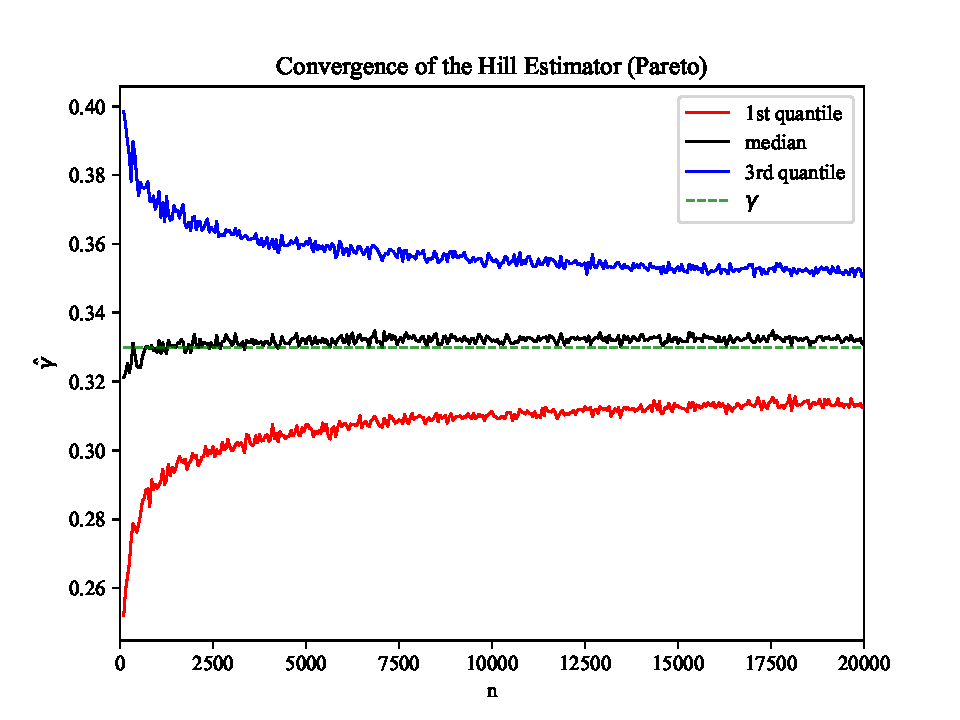
\includegraphics[width=\textwidth]{pareto.pdf}
\caption{A plot of the median, the first quartile and the third quartile of simulated values of the Hill estimator under the Pareto distribution with extreme value index $\gamma=1/3$. The observed quantities are plotted against the sample size. The used threshold was $k(n) = \left\lfloor \sqrt{n} \right\rfloor$ and each sample size was simulated 2000 times. The correct value of the extreme value index is displayed as a dashed line.}
\label{pareto}
\end{center}
\end{figure}

\begin{figure}[H]
\begin{center}
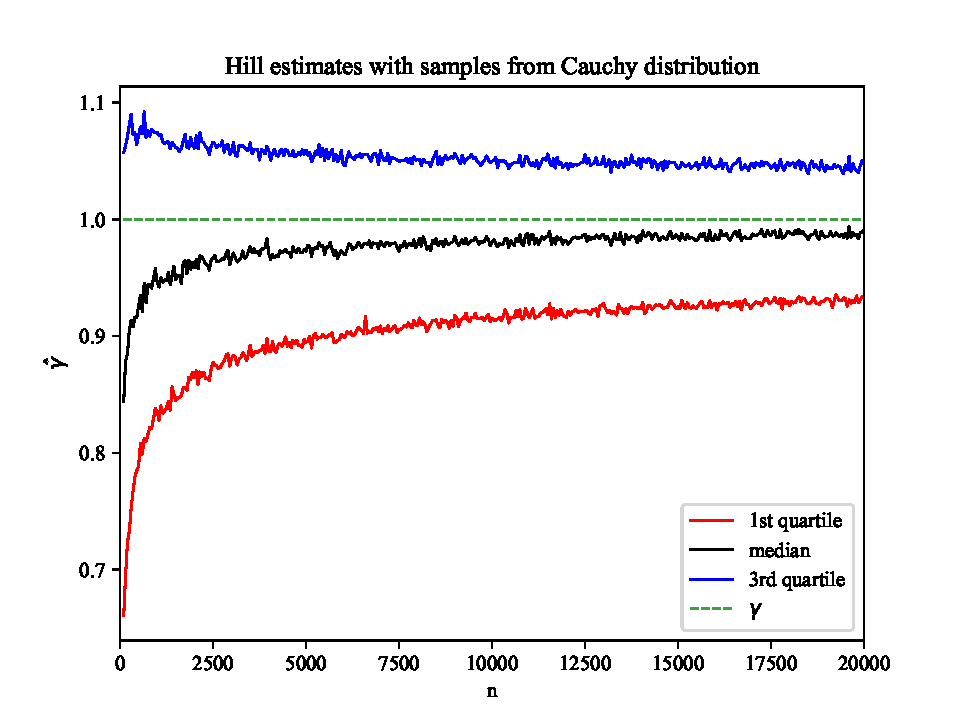
\includegraphics[width=\textwidth]{cauchy.pdf}
\caption{A plot of the median, the first quartile and the third quartile of simulated values of the Hill estimator under the Cauchy distribution. The observed quantities are plotted against the sample size. The used threshold was $k(n) = \left\lfloor \sqrt{n} \right\rfloor$ and each sample size was simulated 2000 times. The correct value of the extreme value index is displayed as a dashed line.}
\label{cauchy}
\end{center}
\end{figure}




\end{document}
